% !TEX TS-program = xelatex

% Inicializace tulthesis
\documentclass[FM]{tulthesis}
% Typografie pro češtinu; xelatex alternativa pro babel
\usepackage{polyglossia}
\setdefaultlanguage{czech}
% Automatické pevné mezery
\usepackage{xevlna}
% Zabránění vdov a sirotků
\usepackage[all]{nowidow}
% Snížit šanci na rozdělení posledního slova odstavce
\finalhyphendemerits=200000
% Umožňuje vytvářet tabulky s vlastními footnotes
\usepackage{threeparttable}
% Zdrojové kódy
% == Zdrojové kódy se syntax highlight ==
\usepackage{listings}
\definecolor{color_base0}{rgb}{0.396078431372549, 0.4823529411764706, 0.5137254901960784}
\definecolor{color_violet}{rgb}{0.4235294117647059, 0.44313725490196076, 0.7686274509803922}
%\definecolor{color_blue}{rgb}{0.14901960784313725, 0.5450980392156862, 0.8235294117647058}
\definecolor{color_green}{rgb}{0.5215686274509804, 0.6, 0}
\definecolor{color_cyan}{rgb}{0.164705882352, 0.6313725490196078, 0.596078431372549}
\lstset{
	, basicstyle = \ttfamily\footnotesize
    , breaklines = true
    , frame = tb
    , commentstyle = \color{color_base0}
    , keywordstyle = \color{color_violet}
    , ndkeywordstyle = \color{color_green}
    , stringstyle = \color{color_cyan}
    , showstringspaces = false
    , prebreak = \raisebox{0ex}[0ex][0ex]{\ensuremath{\hookleftarrow}}
}

%\setmonofont{Courier New}

% Python
\lstdefinelanguage{Python3}[]{Python}{
    morekeywords={async, None},
    morendkeywords={View, add_item, Button, send_message}
}

% JavaScript
\lstdefinelanguage{JavaScript}{
  keywords={new, true, const, async, await},
  ndkeywords={require, module, setName, setDescription, addIntegerOption, setRequired, getInteger, setLabel, setURL, setStyle, addComponents, reply},
  morestring=[b]"
}

% C#
\lstdefinelanguage{Csharp}[Sharp]{C}{
    morekeywords={async, var, await},
    %morendkeywords={Task, SocketSlashCommand, Int64, ComponentBuilder, ButtonStyle, Math}
    morendkeywords={SlashCommandHandler, ElementAt, WithButton, RespondAsync, Pow, Build}
}

% Python
\lstdefinelanguage{Java18}[]{Java}{
    morendkeywords={onSlashCommandInteraction, getName, equals, getOption, getAsInt, reply, addActionRow, queue}
}

% Highlight českých znaků
\makeatletter
\lst@InputCatcodes
\def\lst@DefEC{
	\lst@CCECUse \lst@ProcessLetter
	^^80^^81^^82^^83^^84^^85^^86^^87^^88^^89^^8a^^8b^^8c^^8d^^8e^^8f
	^^90^^91^^92^^93^^94^^95^^96^^97^^98^^99^^9a^^9b^^9c^^9d^^9e^^9f
	^^a0^^a1^^a2^^a3^^a4^^a5^^a6^^a7^^a8^^a9^^aa^^ab^^ac^^ad^^ae^^af
	^^b0^^b1^^b2^^b3^^b4^^b5^^b6^^b7^^b8^^b9^^ba^^bb^^bc^^bd^^be^^bf
	^^c0^^c1^^c2^^c3^^c4^^c5^^c6^^c7^^c8^^c9^^ca^^cb^^cc^^cd^^ce^^cf
	^^d0^^d1^^d2^^d3^^d4^^d5^^d6^^d7^^d8^^d9^^da^^db^^dc^^dd^^de^^df
	^^e0^^e1^^e2^^e3^^e4^^e5^^e6^^e7^^e8^^e9^^ea^^eb^^ec^^ed^^ee^^ef
	^^f0^^f1^^f2^^f3^^f4^^f5^^f6^^f7^^f8^^f9^^fa^^fb^^fc^^fd^^fe^^ff
	^^^^010c^^^^010d% č
	^^00}
\lst@RestoreCatcodes
\makeatother

% Zdrojové kódy uvnitř float
%\usepackage{float}
%\newfloat{lstfloat}{ht}{lop}
%\floatname{lstfloat}{Zdrojový kód}
%\def\lstfloatautorefname{Zdrojový kód}


% Pro seznam použité literatury
\usepackage[backend=biber, style=iso-numeric]{biblatex}
\addbibresource{zdroje.bib}

% Titulní strana
\TULtitle{Tvorba a využití botu pro výuku matematiky na platformě Discord}{Creating and using a bot for teaching mathematics on the Discord platform}
\TULprogramme{B0613A140005}{Informační technologie}{Information technology}
%\TULbranch{B0613A140005AI}{Aplikovaná informatika}{Applied Informatics}
\TULauthor{Radek Mocek}
\TULsupervisor{Ing. Igor Kopetschke}
\TULyear{2024}

% Začátek dokumentu
\begin{document}
	% Prohlášení
	\ThesisStart{male}
	
	% Poděkování
	\begin{acknowledgement}
		Děkuji
	\end{acknowledgement}
	
	% Abstrakt česky
	\begin{abstractCZ}
		Abstrakt česky
	\end{abstractCZ}
	
	% Klíčová slova česky
	\begin{keywordsCZ}
		Klíčová slova česky
	\end{keywordsCZ}
	\vspace{2cm}
	
	% Abstrakt anglicky
	\begin{abstractEN}
		Abstrakt anglicky
	\end{abstractEN}
	
	% Klíčová slova anglicky
	\begin{keywordsEN}
		Klíčová slova anglicky
	\end{keywordsEN}
	
	% Obsah
	\tableofcontents
	
	% Seznam obrázků
	\listoffigures
	
	% Seznam tabulek
	\listoftables
	
	\clearpage
	
	% Zkratky
	\begin{abbrList}
		\textbf{API} & Application Programming Interface, rozhraní pro programování aplikací \\
		\textbf{HTTPS} & \dots \\
		\textbf{JDA} & \dots \\
		\textbf{JSON} & \dots \\
		\textbf{npm} & \dots \\
		\textbf{REST} & \dots \\
		\textbf{SDK} & Software Development Kit, sada nástrojů pro vývoj softwaru \\
		\textbf{VoIP} & Voice over Internet Protocol, telefonie přes internetový protokol \\
		\textbf{UI} & User Interface, uživatelské rozhraní \\
	\end{abbrList}
	
	% Začátek hlavního textu
	
	% 1. Vypracujte rešerši sociálních platforem, které umožňují integraci botů.
	% 2. Analyzujte vybranou skupinu existujících botů na platformě Discord a knihoven pro jejich tvorbu.
	% 3. Navrhněte bot zaměřený na výklad a příklady z lineární algebry při využití specifických funkcí Discordu včetně administrace a interaktivních zpráv.
	% 4. Navržené řešení implementujte a nasaďte do testovacího provozu pro vybranou skupinu uživatelů.
	% 5. Vyhodnoďte zpětnou vazbu od uživatelů a navrhněte případné úpravy a vylepšení.
	
	\chapter{Úvod}
	
	Úvod.
	
	\chapter{Boti na sociálních platformách}
	
	Tato kapitola představuje Discord a některé další sociální platformy, které přímo podporují tvorbu a integraci botů. Nejdříve je ale nutné upřesnit, jak jsou v tomto kontextu myšleny výrazy \textit{sociální platforma} a \textit{bot}.
	
	Discord je vcelku obtížné zařadit do jedné konkrétní kategorie softwaru. Dokud se nově zaregistrovaný uživatel nepřipojí na žádný server, pak se Discord chová jako VoIP a instant messaging aplikace, kde lze komunikovat pouze s lidmi, které si uživatel přidá do přátel. Po připojení na nějaký veřejný Discord server se ale aplikace přibližuje ke kategorii sociálních médií, kdy uživatel může sdílet a konzumovat obsah v rámci moderované komunity. Pojem sociální platforma je zde tedy myšlen spíše jako zastřešující termín pro Discord a jemu podobné aplikace, u nichž o zařazení do této kapitoly především rozhodovalo, zdali nějakým způsobem podporují integraci botů. Společnou vlastností níže zmíněných platforem je také to, že všechny mají k dispozici aplikace pro web, desktop a mobilní zařízení.
	
	Uživatelé sociálních médií často vnímají pojem bot negativně, jelikož se mezi boty mimo jiné řadí i programy generující spam nebo umělou návštěvnost za účelem zkreslení statistik \cite{lit_Discord}. Na platformách zkoumaných v této kapitole je ale bot speciální typ uživatele, jehož chování je automatizované a určené programem. Tento bot je zpravidla přidán do skupinové konverzace, kde pak za pomoci volání API dané platformy dokáže provádět stejné akce jako běžný uživatel. Jedná se například o odesílání zpráv a čtení jejich obsahu, moderaci členů serveru, nebo i připojení do hlasového hovoru. Nemusí se jednat o chatbota, který se snaží imitovat lidské chování. Bot obvykle reaguje na předem danou sadu příkazů vykonáním určité činnosti.
		
	Aby byl bot online a funkční, musí být program, který definuje jeho chování, neustále spuštěný. O tohle se zkoumané platformy zpravidla nestarají, a proto je nutné mít program spuštěný na vlastním serveru nebo využít hosting třetí strany. Tento program pak komunikuje s danou platformou (např. pomocí protokolu \mbox{WebSocket}). Komunikace může být velmi komplexní, proto vznikají komunitní i oficiální knihovny, které tvorbu bota značně usnadňují.
	
	Účet pro bota může být založen v rozhraní pro vývojáře (např. \textit{Discord Developer Portal}), kde je následně vygenerován jeho ověřovací token. Ten se pak používá při komunikaci programu s platformou a měl by zůstat tajný, jinak může dojít k tzv. odcizení bota. To znamená, že někdo jiný použije svůj vlastní program společně s uniklým tokenem pro předefinování chování bota, k jehož účtu daný token náleží.
	
	\section{Discord}
	
	Platforma Discord vznikla v roce 2015 jako reakce na nedostatky tehdejších služeb pro online komunikaci mezi hráči videoher \cite{lit_Discord}. S nabývající popularitou se ale na Discordu začaly objevovat veřejné komunity zaměřené i na jiná témata, než ta herní. Často se jedná o oficiálně vytvořené servery patřící k nějakému produktu, které slouží jako diskuzní fórum a propagace zároveň. Momentálně je například největší komunitou (podle počtu členů) server Midjourney, který patří ke stejnojmennému nástroji pro tvorbu obrázků pomocí umělé inteligence. Uživatelé zde mohou o nástroji diskutovat, hlásit chyby, sdílet vytvořené obrázky, nebo je nechat generovat použitím Midjourney bota.
	
	Základní verze Discordu je zdarma s možností měsíčního předplatného \textit{Discord Nitro}. Předplatitelé mají navíc k dispozici kosmetické prvky (např. vlastní emotikony nebo animovaný avatar) a některé základní funkce jsou pro ně vylepšeny (např. nahrávání větších souborů nebo streamování videa ve vyšším rozlišení).	

	Program disponuje obvyklou instant messaging a VoIP funkcionalitou. V tzv. přímých zprávách si mezi sebou uživatelé mohou posílat textové zprávy a soubory. Dále je k dispozici hlasový hovor s případným sdílením obrazovky nebo videa z webkamery. Tyto akce lze provádět i v soukromých skupinách, které ale mají omezený počet deseti uživatelů. Textové zprávy je možné formátovat v jazyce Markdown (např. tučný text, nadpisy, seznamy, zdrojové kódy se zvýrazněním klíčových slov).
	
	Discord server (interně zvaný \textit{guild}) je izolovaná kolekce uživatelů a kanálů \cite{doc_Discord}. Kanály jsou nejčastěji textové nebo hlasové a funkčně odpovídají komunikaci v soukromé skupině. Rozdíl je ten, že komunikace v kanálu se mohou účastnit všichni členové daného serveru (kterých může být v základu až 500~000), kteří k tomu mají dostatečná oprávnění. Členům serveru lze přiřazovat tzv. role, u kterých se pak tato oprávnění nastavují (např. všichni uživatelé s rolí $x$ mohou číst historii zpráv v kanále $y$).
	
	\subsection{Aplikace a boti}
	
	Jako Discord aplikace se označuje vše, co oficiálně komunikuje s Discord API. Bot je pak automatizovaný uživatel, který může být k aplikaci přidán. Od roku 2021 jsou preferovanou metodou ovládání bota příkazy začínající lomítkem. Seznam těchto tzv. podpůrných příkazů (\textit{slash commands}) se synchronizuje s Discordem a díky tomu je pak k dispozici jejich našeptávání. Namísto příkazu umí bot reagovat i na události (např. uživatel klikl na tlačítko nebo se připojil na server). Botem odeslané zprávy pak mohou obsahovat interaktivní prvky jako tlačítko, výběrový seznam a textové pole. Je také možné vyvolat vyskakovací okno obsahující tyto prvky. Kromě práce se zprávami může bot také upravovat nastavení serveru nebo se připojit do hlasového hovoru. \cite{pdf_apps101}
	
	\begin{figure}[ht]
		\centering
		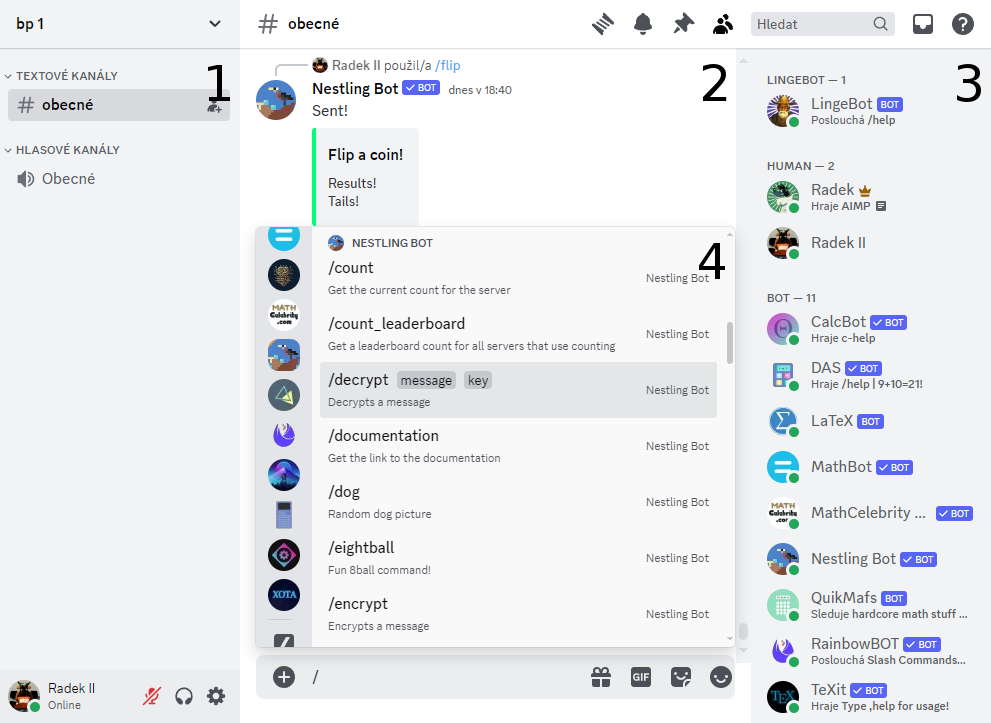
\includegraphics[width=\textwidth]{img/DiscordBotCommands}
		\caption{Discord: Uživatelské rozhraní a použití bota}
	\end{figure}
	
	Boti tedy operují především na serverech\footnote{Boty lze ale používat i v přímých zprávách. Bot se sice tváří jako uživatel, do přátel ho ale přidat nelze a pro zahájení přímé konverzace je nutné s ním nejdříve mít nějaký společný server. Bota nelze přidat do soukromé skupiny.} a existuje několik možností, jak je na nějaký server pozvat. Na konci roku 2022 byl do Discordu přidán tzv. adresář aplikací (\textit{App Directory}), který momentálně obsahuje seznam více než 5500 dostupných botů, kde každý z nich má svou stránku s podrobnějším popisem a tlačítkem pro přidání na server. Aby byl bot v tomto adresáři obsažen, musí nejprve projít schvalovacím procesem, a proto se jich zde nachází pouze zlomek ze všech existujících. Každý bot pak má svůj speciální zvací odkaz (\textit{bot invite link}) a existuje několik neoficiálních databází (např. \href{https://top.gg}{top.gg}), které opět obsahují seznam botů s jejich popisem a zvacím odkazem. Poslední možností jsou boti s otevřeným zdrojovým kódem, které si uživatel stáhne a spustí na vlastním stroji. Tento způsob vyžaduje botu založit účet a vygenerovat vlastní token.
	
	Discord boti nabízející nástroje pro usnadnění moderace zejména na velkých serverech patří mezi ty nejpoužívanější. Obvykle mají svou stránku s administrací, kde si lze např. zobrazit statistiky serveru, nastavit automatické přivítání a přiřazení rolí novým členům, vyhození za spam apod. Oblíbenou kategorií byli také hudební boti, kteří v hlasovém hovoru pouštěli vybrané skladby. Jejich popularita klesla roku 2021, kdy Google zakázal provoz botů přehrávajících hudbu z webu \mbox{YouTube}. Další častá kategorie botů jsou hry a zábava. Jedná se buď o boty poskytující jednoduché hry v prostředí textového chatu, nebo propojující nějakou existující videohru s Discordem.
	
	\section{Slack}
	
	Z populárních platforem se Discordu vzhledově i funkčně nejvíce podobá program Slack. Ten byl spuštěn již v roce 2013 a od té doby si vybudoval reputaci jako standard pro komunikaci v technologických společnostech. \cite{lit_Discord}
	
	Slack se prezentuje jako software usnadňující interní komunikaci v organizacích a dal by se nazvat jako \quotedblbase Discord pro firmy\textquotedblleft. Namísto serverů jsou zde tzv. workspaces. Workspace má své členy a textové kanály, ve kterých lze zahájit i hlasový hovor. Členové jednoho workspace si mezi sebou mohou posílat přímé zprávy a pomocí funkce \textit{Slack Connect} je možné komunikovat i s lidmi z jiného workspace. Na rozdíl od Discordu, kde jsou přímé zprávy kompletně oddělené od ekosystému serverů, se zde všechny prováděné akce dějí uvnitř nějakého workspace.
	
	Slack má k dispozici několik úrovní měsíčního předplatného a verze zdarma je značně omezena. V bezplatné verzi nelze např. zobrazit zprávy starší než 90 dnů a provozovat hlasový hovor ve více než dvou lidech. Omezené je i použití tzv. aplikací.
	
	Zdejší aplikace (\textit{Apps}) se podobají zkoumaným botům a jejich výběr odpovídá cílové skupině Slacku. Zaměřují se především na zvýšení produktivity, \mbox{teambuilding}, nebo integraci již existující služby třetí strany do prostředí Slacku. Stejně jako uživatelé mohou Slack aplikace spravovat konverzace a odesílat do nich textové zprávy. Ovládání aplikací probíhá buď pomocí příkazů začínajících lomítkem, nebo má každá aplikace svou domovskou stránku a může také generovat vyskakovací okna. Aplikací odeslané zprávy, její domovská stránka a vyskakovací okna mohou obsahovat širokou škálu interaktivních prvků (tlačítko, zaškrtávací pole, výběr data a času apod.).
	
	\begin{figure}[ht]
		\centering
		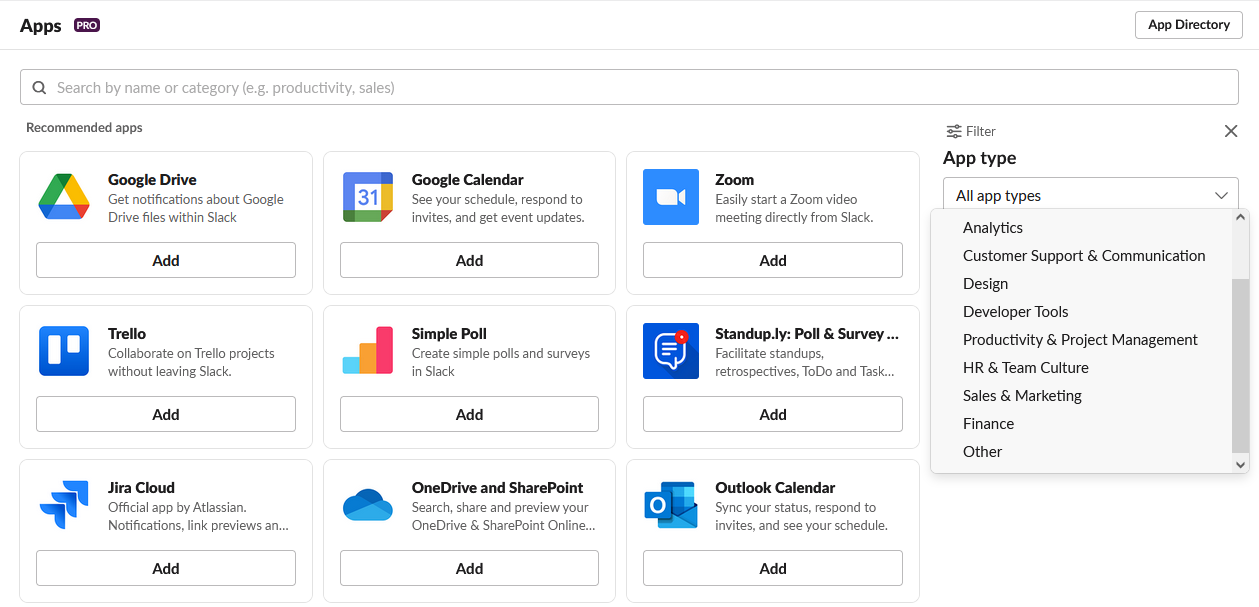
\includegraphics[width=\textwidth]{img/SlackApps}
		\caption{Doporučené Slack aplikace}
	\end{figure}
	
	Zorientovat se v procesu tvorby Slack aplikací nemusí být jednoduché. Tyto aplikace se totiž dělí na klasické (\textit{classic}) a nové (zvané \textit{modern} nebo \textit{next-generation}, představené v roce 2021), jejichž API se liší. Ani slovo bot není ve Slack ekosystému jednoznačné. U klasických aplikací se jedná o jejich speciální typ, se kterým je komunikace vedena běžnou řečí namísto příkazů nebo UI (chatbot). Tento bot je označen jako \textit{legacy} a v budoucnu pravděpodobně nebude podporován. U nového typu aplikací se z pohledu uživatele slovo bot nikde nevyskytuje (maximálně v názvu nějaké aplikace), z dokumentace je ale zjevné, že se (stejně jako u Discordu) jedná o speciálního uživatele ovládaného danou aplikací, tato informace však není nikde explicitně zmíněna. Při práci s dokumentací nebo neoficiálními návody je tedy nutné dávat pozor na to, s jakou technologií daný manuál pracuje, protože může dojít ke snadné záměně výše zmíněných pojmů.
	
	Klasické Slack aplikace lze vyvíjet v řadě komunitních knihoven. \textit{Next-generation apps} pak mají připravené oficiální \mbox{TypeScript} SDK a o hosting se stará přímo Slack, pro jejich vývoj a následné nasazení je ale nutné mít placenou verzi Slacku.
	
	\section{Guilded a Revolt}
	
	Guilded a Revolt jsou platformy, které jsou přímo inspirované Discordem a podobnost mezi nimi je nepřehlédnutelná. Ekosystém uživatelů, přímých zpráv, serverů a botů je u těchto tří platforem takřka identický. Guilded ani Revolt nemají ekvivalent k podpůrným příkazům. Boti tedy musí kontrolovat obsah každé odeslané zprávy na serveru, jestli neobsahuje nějaký z jejich příkazů. Každý bot má obvykle svůj prefix (např. vykřičník) a problém nastává, když má více botů stejný prefix a příkaz se stejným názvem (např. po napsání \quotedblbase!help\textquotedblleft\ do chatu zobrazí svou nápovědu všichni takoví boti)\footnote{Tímto způsobem se před představením podpůrných příkazů ovládali i boti na Discordu. Problém stejných příkazů se řešil buď víceznakovými prefixy (menší šance na kolizi), nebo nastavitelným prefixem (to vyžaduje nějaké úložiště uchovávající dvojice id serveru a prefix). Tento starý typ příkazů lze stále používat např. pokud je vývojář chce skrýt před běžnými uživateli (tyto příkazy se neobjeví v našeptávači).}. Obě platformy mají oproti Discordu znatelně menší uživatelskou základnu a počet jejich veřejných botů se pohybuje v řádu desítek.
	
	Guilded (2017) lze považovat za konkurenci Discordu, která se zaměřuje na jeho původní účel. Tím je komunikace pro hráče videoher. Guilded přidává funkce užitečné pro pořádání pravidelných komunitních událostí. Uživatel zde také může propojit svůj účet s vybranými herními tituly. \cite{web_guilded} 
	
	Program je zdarma, ale správci mohou na svém serveru zapnout dobrovolné měsíční předplatné, ze kterého je část odváděna Guilded. Pro tvorbu botů lze využít komunitních knihoven.
	
	Revolt (2021) je Discord alternativa s otevřeným zdrojovým kódem. Oproti konkurenci nemá Revolt žádné speciální funkce, díky tomu je ale méně komplikovaný. Kromě řady komunitních knihoven pro tvorbu botů je k dispozici i oficiální revolt.js. Tato knihovna byla vytvořena tak, aby do ní šel snadno migrovat bot napsaný v knihovně discord.js.
	
	\section{Další platformy}
	
	Do této sekce byly zařazeny další sociální platformy, které sice podporují implementaci botů ve smyslu automatizovaných uživatelů, ale oproti výše zmíněným platformám mají buď znatelně odlišnou strukturu a uživatelské rozhraní, nebo menší uživatelskou základnu, která se pak projevuje i v malém počtu existujících botů a malé komunitě kolem knihoven pro jejich tvorbu.
	
	\subsection{Matrix}
	
	Matrix je otevřený protokol pro šifrovanou a decentralizovanou komunikaci po síti. Existuje pro něj několik klientských aplikací (např. Element) a poskytovatelů (např. matrix.org). Protokol je také možné provozovat na vlastním serveru. Komunikace zde probíhá v tzv. místnostech. Místnost je jeden textový kanál s možností zahájení hlasového hovoru, který může být soukromý i veřejný. Pak jsou zde tzv. prostory, které jsou v podstatě jen spravované seznamy různých místností. Podle dokumentace jsou prostory podobné Discord serverům nebo Slack workspaces, avšak zde připojení do prostoru uživatele automaticky nepřipojí do všech místností (uživatel si může vybrat, kam se připojí) a místnosti nejsou na prostorech závislé (místnost může existovat bez prostoru, může ale být i součástí více prostorů). Matrix podporuje komunikaci uživatelů s různými poskytovateli tohoto protokolu ve stejné místnosti.
	
	Bot zde není speciálním typem uživatele, ale je pro něj zaregistrován běžný uživatelský účet. Program s logikou bota tedy může ovládat jakýkoliv účet (pokud zná jeho přístupový token)\footnote{V terminologii Discordu se běžné uživatelské účty řízené programem nazývají \textit{self-bots} a jejich provoz porušuje podmínky používání.}. Pro tvorbu takovýchto botů je připraveno oficiální \mbox{TypeScript} SDK. Veřejných botů pro Matrix není mnoho, mezi populární boty ale patří i boti modulární, do nichž mohou ostatní vývojáři přidávat vlastní funkcionalitu.
	
	Specifickou vlastností Matrixu jsou mosty (\textit{bridges}). Ty umožňují propojit místnost s nějakou jinou platformou (např. Discord, Slack nebo Messenger). Chat z platformy třetí strany by se pak měl zrcadlit s vybranou místností. Uživatelé z jiné platformy mají v Matrix místnosti svou reprezentaci zvanou \textit{ghost}. Pokud to daná platforma podporuje, tak v jejím ekvivalentu místnosti budou uživatelé ze strany Matrixu reprezentováni jako tzv. \textit{puppets}. \cite{doc_Matrix}
	
	\subsection{Microsoft Teams}
	
	Microsoft Teams je, stejně jako Slack, platforma pro firemní komunikaci. Každý účet na Teams náleží jedné organizaci (přihlašuje se obvykle přes firemní e-mail). Organizace se pak dělí na týmy, které se mohou dělit na kanály. Tým je kolekce uživatelů, která by měla reprezentovat určitý celek v dané organizaci (např. lidé pracující na konkrétním projektu). Kanály jsou sekce svého týmu, ve kterých probíhá komunikace ve formě příspěvků a komentářů. Klasický textový chat s případným hlasovým hovorem probíhá v samostatné sekci a umožňuje se spojit i s uživateli z jiné organizace.
	
	Podobně jako u Slacku se zdejší aplikace zaměřují především na zvýšení produktivity a propojení Teams s dalšími službami. Bot je v Teams terminologii aplikace vykonávající repetitivní úkony, která se může účastnit konverzace v chatu nebo kanálu. Boti se tvoří v oficiálním SDK (jazyky C\#, JavaScript, Python). Na konci roku 2023 bylo představeno Microsoft Copilot Studio, které mimo jiné podporuje tvorbu Teams botů pomocí grafického rozhraní bez psaní zdrojového kódu. Pro tento typ botů není potřeba vlastní hosting.
	
	Platforma Teams je součástí předplatného Microsoft 365. Existuje i bezplatná verze, ta má ale omezenou funkcionalitu a nedovoluje integraci aplikací (včetně botů). Kromě Teams pro firmy byla také později představena verze pro domácnosti. Ta by měla sloužit pro komunikaci s rodinou a přáteli. Většina funkcí je v této verzi vypnuta. Místo týmů jsou zde tzv. komunity, které se chovají totožně, pro jejich správu je ale nutné použít mobilní aplikaci.
	
	\subsection{Flock}
	
	Flock je platforma pro firemní komunikaci, která podle svého webu nabízí oproti konkurenčnímu Slacku a Teams více funkcí za méně peněz. Tento web obsahuje výčet více jak sta vlastností, ve kterých je Flock údajně lepší než konkurence. Po bližším průzkumu je ale zjevné, že některá uvedená tvrzení jsou nepravdivá nebo zavádějící.
	
	Struktura Flocku je podobná jako u ostatních platforem: Jednotlivé servery se nazývají týmy a obsahují textové kanály, ve kterých je možné zahájit hlasový hovor. Zdejší aplikace komunikují s Flock API a boti jsou jejich uživatelské reprezentace. Výběr aplikací je podobný jako u platforem Slack a Teams.
	
	Platforma pro vývoj Flock aplikací se nazývá FlockOS a má slogan \quotedblbase World's First Chat Operating System\textquotedblleft, s operačním systémem ale nemá nic společného. Boty lze programovat v oficiálním SDK, jehož poslední verze ale vyšla v roce 2017.
	
	\subsection{Mattermost, Rocket.Chat a Zulip}
	
	Mattermost, Rocket.Chat a Zulip jsou komunikační platformy s otevřeným zdrojovým kódem. Díky tomu je možné provozovat tyto platformy na vlastních strojích (self-hosting), což je vhodné pro firmy, které díky tomu mají všechna data z chatů uložena u sebe. Všechny tři platformy ale nabízí i svůj hosting v několika úrovních měsíčního předplatného. Struktura těchto programů se pak podobá Slacku.
	
	Mattermost nemá žádnou knihovnu pro tvorbu botů, veškerou logiku komunikace s jejich API tedy musí zajistit vývojář bota. Pro Rocket.Chat je možné vyvíjet boty v oficiálním JavaScript SDK, nebo je vytvořit v grafickém rozhraní na platformě Botpress. Zulip má pro vývoj botů k dispozici oficiální Python knihovnu.
		
	\chapter{Matematika na platformě Discord}
	
	Ze zkoumaných sociálních platforem má Discord nejkomplexnější a nejlépe zdokumentovaný ekosystém botů. Kolem tvorby těchto botů vznikla početná komunita a existuje pro ni tedy i nejvíce knihoven. Discord nemá žádné specifické zaměření (např. firemní nebo herní) a díky tomu pokrývá širokou škálu uživatelů. Proto byla pro tvorbu matematického bota vybrána právě tato platforma.
	
	Ačkoliv nebyl Discord vytvořen pro účely výuky a nemá žádné speciální matematické nástroje, \textit{vzdělávání} je jednou z pěti hlavních kategorií veřejných Discord serverů a patří do ní i servery specializované na matematiku. \textit{Mathematics} je nejpopulárnější server s tímto zaměřením, na kterém mohou uživatelé diskutovat a řešit matematické problémy různých úrovní složitosti.
	
	Na serveru je také automatický systém přiřazování textových kanálů uživatelům s konkrétním matematickým problémem. Ostatní uživatelé se v daném kanále mohou pokusit zadaný problém vyřešit. Jakmile je zadavatelova otázka zodpovězena, textový kanál se může použít pro problém dalšího uživatele. O logiku přiřazování kanálů se stará místní bot.
	
	Matematicky zaměřených Discord botů není mnoho. V oficiálním adresáři aplikací nebyl během rešerše nalezen žádný. V neoficiálních databázích pak sice bylo nalezeno několik desítek botů, kteří se podle popisu alespoň částečně zabývají matematikou, velká část z nich ale byla offline a neměla k dispozici zdrojový kód. Otestováno bylo tedy nakonec 11 botů, které lze zařadit do dvou kategorií.
	
	\section{Bot vykreslující matematické výrazy}

	Jelikož Discord nemá žádnou podporu pro vykreslování matematických výrazů, což je v textové konverzaci ohledně matematiky velmi užitečné, existuje hned několik botů s touto funkcionalitou. Konkrétně vykreslení umožňuje 5 z 11 testovaných botů. K popisu výrazu se ve všech případech používá TeX syntax, ve které je zadán vstupní parametr vykreslovacího příkazu. Bot pak podle parametru vygeneruje obrázek s matematickým výrazem a odešle ho do textového kanálu, kde byl příkaz zadán.
	
	Dva zkoumaní boti mají možnost zapnout automatické vykreslování: Jakmile jakákoliv odeslaná zpráva na serveru obsahuje dvakrát symbol dolaru, bot celou tuto zprávu vykreslí do obrázku a text mezi dolary nahradí matematickým zápisem (obrázek \ref{_tag_img_autotex}). Tři boti pak umožňují změnit barevné schéma generovaných obrázků. Je vhodné, aby tyto obrázky neměly průhledné pozadí, jinak by např. uživatelé používající světlý motiv Discordu nemohli přečíst text v obrázcích s bílou barvou písma (na průhledném pozadí).
	
	\begin{figure}[ht]
		\centering
		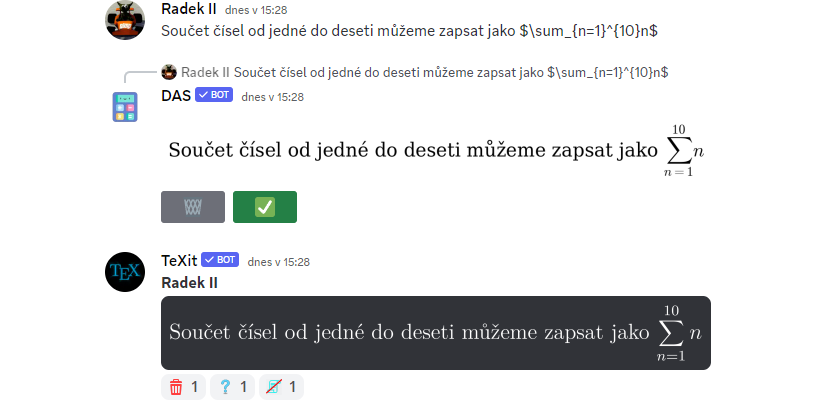
\includegraphics[width=\textwidth]{img/AutoTeX}
		\caption{Automatické vykreslení matematického výrazu}
		\label{_tag_img_autotex}
	\end{figure}
	
	U botů psaných v jazyce JavaScript lze pro implementaci této funkcionality využít knihovny KaTeX nebo MathJax. V jazyce Python to pak umožňuje Matplotlib. Tento balík sám o sobě ale neumí vykreslovat složitější prvky jako např. matice. K tomu je potřeba, aby na stroji, kde je bot spuštěn, byla nainstalována LaTeX distribuce, která se pak použije namísto výchozího Matplotlib vykreslování. Další možností nezávislou na použitém jazyku či knihovně je využít pro vykreslení nějakou externí službu.
	
	\section{Bot jako kalkulačka}
	
	Celkem devět otestovaných botů má jeden nebo více příkazů pro výpočet jednoduchých příkladů. V lepším případě se jedná o jeden příkaz (typu \textit{vypočti}), kterému se jako vstupní parametr zadá příklad s různými operacemi (včetně závorek, goniometrických funkcí apod.) a výstupem je výsledek celého výrazu. Velmi nepraktickou variantou jsou pak boti se sadou příkazů pro různé operace (typu \textit{sečti}, \textit{vynásob}, \dots), kde vstupem je několik čísel.
	
	Kromě výpočtu numerických příkladů se také objevují příkazy např. pro úpravy výrazů, derivace apod. Sedm botů pak dokáže vygenerovat obrázek s jednoduchým grafem dle zadaného předpisu. Dva boti umí zadat uživatelův vstup do služby Wolfram Alpha a do chatu odeslat její výstup.
	
	Jeden bot dokáže generovat náhodné příklady, jedná se ale pouze o čtyři základní binární operace. Tedy např. $x+y$, kde $x$ a $y$ jsou v rozmezí 1 až 99. Bot postupně generuje sérii deseti příkladů a uživatel má u každého deset vteřin na zadání výsledku. Po dokončení série příkladů je pak uživateli zobrazeno jeho skóre.
	
	% \section{DAS} ?
	
	\chapter{Prostředky pro tvorbu Discord bota}
		
	Discord API, se kterým program ovládající bota komunikuje, se dělí na dvě hlavní vrstvy: Pro obecné operace slouží HTTPS REST API a pro odesílání a přihlašování k událostem v reálném čase se používají trvalá zabezpečená připojení pomocí protokolu WebSocket. Samotná komunikace pak probíhá ve formátu JSON a pro unikátní identifikátory všech objektů se využívá formát Twitter Snowflake ID.	Discord operuje na tak velkém měřítku, že zajistit úplnou konzistenci jeho dat by bylo nemožné, a proto je většina operací v Discord API eventuálně konzistentní. \cite{doc_Discord}
	
	Eventuální konzistence znamená, že distribuovaná a replikovaná databáze povoluje relativně velké množství nekonzistentních dat. Pokud ale po nějaký čas neproběhne operace zápisu, tak se data na všech replikách postupně \quotedblbase srovnají\textquotedblleft. \cite{book_distributedSystems4}
	
	Tvorba aplikací pracujících nad eventuálně konzistentními daty může být náročná. Události z Discord API navíc nemusí klientovi vždy přijít právě jen jednou, a proto je na ně nutné reagovat idempotentně. Výsledek několikrát provedené idempotentní operace by měl být stejný, jako kdyby byla provedena jen jednou. \cite{book_distributedSystemsUnderstanding}
	
	Z důvodu usnadnění tvorby Discord botů začaly pro tento účel vznikat komunitní knihovny. Oficiální dokumentace jich zmiňuje celkem 21 pro 11 různých programovacích jazyků. Tato sekce blíže představuje některé z těchto knihoven, ve kterých byl v rámci rešerše implementován jednoduchý příkaz pojmenovaný \textit{pow}. Ten přijímá dva celočíselné parametry, se kterými provede umocňování. Ke zprávě s výsledkem je ještě přidáno tlačítko \textit{Example} odkazující na webovou stránku (obrázek \ref{_tag_img_pow}).
	
	\begin{table}[ht]
		\centering
		\caption{Nejpopulárnější knihovny pro tvorbu Discord botů}\medskip
		\begin{threeparttable}
			\begin{tabular}{ l l r r }
				\textbf{Název} & \textbf{Jazyk} & \textbf{Vznik} & \textbf{Popularita}\tnote{*} \\\hline
				discord.js	& JavaScript 	& 2015 & 24 452 \\
				discord.py	& Python		& 2015 & 14 024 \\
				DiscordGo	& Go			& 2015 & 4 563 \\
				serenity	& Rust			& 2016 & 4 259 \\
				JDA			& Java			& 2015 & 4 038 \\
				Discord.Net & C\#			& 2015 & 3 165 \\
				Pycord		& Python		& 2021 & 2 619 \\
				Discord4J	& Java			& 2015 & 1 697 \\
				Eris		& JavaScript	& 2016 & 1 465 \\
				DSharpPlus	& C\#			& 2016 & 1 179 \\
			\hline\end{tabular}
			\begin{tablenotes}
				\item[*] počet GitHub hvězd ke dni 15. 2. 2024
			\end{tablenotes}
		\end{threeparttable}
	\end{table}
	
	\section{discord.py}
	
	Discord.py je knihovna pro tvorbu Discord botů v jazyce Python (verze 3.8 a vyšší), která je distribuována v podobě balíku instalovaného programem pip. Pro definici veškeré funkcionality bota se využívá klíčových slov \verb*|async| a \verb*|await|. Bot je zde instancí předdefinované třídy s metodami, které se spouští při určité události a jejichž tělo lze dodefinovat. Pro přiřazení metod ke konkrétní události se často používají dekorátory (syntax umožňující upravit chování metod bez zásahu do jejich těla). Některé části discord.py (např. interaktivní prvky nebo tzv. \textit{cogs}) pak využívají objektového návrhu. Díky cogs lze tvořit bota modulárně (rozdělit zdrojový kód do více souborů).
	
	Výhodou discord.py je jeho velká komunita, od které lze získat podporu např. na webu Stack Overflow nebo na oficiálním Discord serveru této knihovny. Díky použití dekorátorů (a jazyku Python obecně) může být psaný kód čistý a přehledný. Pro definici příkazů lze navíc využít anotací a komentářů u příslušných metod. Knihovna má k dispozici referenční příručku, která stručně popisuje veškerou její funkcionalitu. Podrobnější popisy nebo příklady použití se zde ale vyskytují jen zřídka.
	
	Největším problémem discord.py je podle hlasování uživatelů na GitHub \mbox{Issues} právě absence uživatelské příručky. Referenční příručka je dobrým nástrojem hlavně pro programátory, kteří už obecnou tvorbu botů v této knihovně ovládají, a neobsahuje např. informace o tom, jak strukturovat větší projekt nebo co znamenají jednotlivé funkce v kontextu Discordu (z pohledu uživatele).
	
	V roce 2021, kdy byly mimo jiné představeny podpůrné příkazy, vyšla nová verze Discord API, která přinesla zásadní změny v jeho používání. To vedlo k frustraci autorů některých knihoven a vývoj discord.py byl pozastaven. Po šesti měsících se repozitář opět otevřel a vývoj mohl pokračovat, mezitím ale vzniklo několik nových knihoven založených na discord.py (konkrétně Pycord, Nextcord a disnake). Zároveň začaly vycházet balíky, které do existující knihovny přidávaly podporu pro novou verzi Discord API. Zdrojové kódy těchto knihoven jsou si velmi podobné, a proto je při hledání informací nutné dávat pozor na to, s jakou knihovnou daný zdroj pracuje.
	
	\section{discord.js}
	
	Discord.js je knihovna pro běhové prostředí Node.js umožňující tvorbu Discord botů v jazycích JavaScript nebo TypeScript. Funkcionalita je založena na objektech \verb*|Promise| a při psaní kódu se využívá tzv. arrow funkcí. Režie pro zprovoznění podpůrných příkazů a modularity (zde ve stylu \textit{co soubor, to příkaz}) je o něco složitější než u discord.py.
	
	Velkou výhodou této knihovny je existence uživatelské příručky, která programátora provede krok za krokem od úvodní instalace npm balíčku až po tvorbu pokročilých příkazů. Krom popisu postupů a zdrojových kódu se díky tomuto návodu programátor rychle dozví, co všechno do svého bota vlastně může implementovat. Nechybí ani referenční příručka a početná komunita jako u discord.py.
	
	Knihovna nevyužívá dekorátorů ani komentářů pro definování příkazů. Výsledný kód obsahuje mnoho vnořených nebo zřetězených funkcí, kvůli kterým může být delší a hůře čitelný. Knihovna sice podporuje TypeScript, oficiálních ani komunitních návodů pro jeho korektní použití ale není mnoho.
	
	\section{Discord.Net}
	
	Discord.Net je knihovna pro tvorbu Discord botů na platformě .NET distribuovaná přes systém NuGet. Dokumentace je psaná pro jazyk C\# (ve kterém je tato knihovna implementována), je ale možné použít i jiné jazyky z této platformy (např. F\# nebo Visual Basic). Knihovna má k dispozici referenční i uživatelskou příručku, její nevýhodou je menší komunita.
	
	 Pro tvorbu složitějších botů se doporučuje použít vkládání závislostí\footnote{Vkládání závislostí (\textit{dependency injection}) je návrhový vzor, kde se třetí strana stará o vztahy mezi komponentami a jejich závislostmi (aby byla za běhu programu do vybraných atributů dosazena správná instance) \cite{lit_distributedSystems}. Zde se konkrétně jedná o balík \textit{Microsoft.Extensions.DependencyInjection}.}. Oproti předchozím knihovnám Discord.Net u podpůrných příkazů odděluje logiku jejich synchronizace a obsluhy. Kód zde tedy není strukturován na metody odpovídající jednotlivým příkazům, ale všechny příkazy jsou obsluhovány jedinou metodou, ve které je kód dále rozvětven\footnote{Podpůrné příkazy musí být synchronizovány, aby je mohli uživatelé používat. V discord.py a discord.js jsou všechny potřebné informace pro synchronizaci (jméno, popis, a vstupní parametry) součástí definice obslužné funkce daného příkazu. V Discord.Net jsou tyto informace uvedeny ve speciální metodě pro synchronizaci. Druhá speciální metoda pak obsluhuje všechny příkazy. Obvykle je uvnitř této metody rozvětvení typu \textit{switch} podle jména příkazu.}.
	
	\section{JDA}
	
	JDA je knihovna pro tvorbu botů v jazyce Java nebo Kotlin. Do projektu je přidána pomocí nástroje Maven nebo Gradle. Stejně jako u Discord.Net je zde oddělená logika synchronizace podpůrných příkazů s Discordem a jejich samotné obsluhy.
	
	Referenční příručka JDA je vygenerována přes Javadoc, což může být vhodné pro programátory zvyklé na jazyk Java, dokumentace ale působí složitě a nepřehledně. K dispozici je také uživatelská příručka včetně ukázkové implementace bota přehrávajícího hudbu v hlasovém hovoru. Ze čtyř zkoumaných knihoven se jedná o jedinou, která by takto v návodu obsahovala krok za krokem kompletní proces tvorby bota s konkrétním zaměřením.
	
	\chapter{Tvorba matematického Discord bota}
	
	\section{Návrh}
	 
	% todo Separate Literals etc. (db_io + premissions) in code ?
	
	\section{Implementace}
	
	% Problém testování nových funkcí u již nasazeného bota, udělat druhého ? (pak je problém slash commands sync (to by mohly řešit hybridní příkazy (u nich je ale problém ctx vs itx ?)))
	
	\section{Zhodnocení}
	
	\chapter{Závěr}
	
	Závěr. //TODO slova rozdělená na dvě stránky%todo
	
	% Zdroje
	\chapter*{Seznam použité literatury}
	\addcontentsline{toc}{chapter}{Seznam použité literatury}
	\printbibliography[heading=none]
	
	% Přílohy
	\appendix
	\chapter{Přílohy}
	
	\section{Zdrojové kódy implementace ukázkového příkazu}
	
	\begin{figure}[ht]
		\centering
		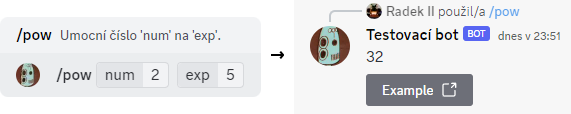
\includegraphics[width=\textwidth]{img/ExampleCommand}
		\caption{Ukázkový příkaz}
		\label{_tag_img_pow}
	\end{figure}
	
	\begin{figure}[ht]
		\lstinputlisting[language=Python3]{code/discord.py}
		\caption{Ukázkový příkaz: Implementace v discord.py}
	\end{figure}
	
	\begin{figure}[ht]
		\lstinputlisting[language=JavaScript]{code/discord.js}
		\caption{Ukázkový příkaz: Implementace v discord.js}
	\end{figure}
	
	\begin{figure}[ht]
		\lstinputlisting[language={CSharp}]{code/discord.cs}
		\caption{Ukázkový příkaz: Implementace v Discord.Net}
	\end{figure}
	
	\begin{figure}[ht]
		\lstinputlisting[language={Java18}]{code/discord.java}
		\caption{Ukázkový příkaz: Implementace v JDA}
	\end{figure}
	
\end{document}